% fig4_architecture_dimensional.tex
%
% What DarwinDiff actually is, with the spatial dimension left IN.
%
% An earlier version drew a scalar MLP: two inputs, one output. That is wrong in the one way
% that matters. The network runs PER CELL over a field, and per-cell structure is
% load-bearing -- the global-scalar control holds the trio at 0/50 against 25/50. A flat MLP
% erases exactly the thing the result depends on.
%
% COLOUR CARRIES ROLE, and only three roles exist:
%   green  = real, measured, not ours          (forcing in, observations out)
%   blue   = the model                          (network, parameter field, box)
%   orange = a CHOICE we made                   (the collapse)
%   red    = reserved for the gradient, nothing else
% An earlier draft used green twice for different things and red for the parameter field,
% which put it in competition with the gradient. One hue, one meaning.
%
% LAYOUT IS ON A GRID, not eyeballed:
%   stage centres  x = 0, 2.6, 5.2, 7.8, 10.4, 13.0   (even 2.6 pitch)
%   flow baseline  y = 0        headings y = 1.18      captions y = -1.05
%   callouts       y = 2.40, equal width, both anchored to the stage they annotate
% Slabs are centred on their anchor (grid drawn -2..2) so a stage centre is a real centre.
%
% ---------------------------------------------------------------------------------------
% TECHNIQUE ADAPTED, WITH THANKS:
%   isometric cell sheet, after the cuboid pics in
%     PetarV-/TikZ X-CNN         https://github.com/PetarV-/TikZ/tree/master/X-CNN
%   palette mixed toward black, one hue -> text/draw/fill triple, after
%     tikz.net "Neural networks" https://tikz.net/neural_networks/
% Framing follows BINN (Xu et al., Geosci. Model Dev. 19, 6777, 2026), which pairs a neural
% parameter map with a process model end to end. doi:10.5194/gmd-19-6777-2026
% ---------------------------------------------------------------------------------------
%
%   pdflatex fig4_architecture_dimensional.tex
%
\documentclass[tikz,border=10pt]{standalone}
\usetikzlibrary{arrows.meta,positioning,calc,fit,backgrounds}

\colorlet{myblue}{blue!80!black}
\colorlet{mygreen}{green!55!black}
\colorlet{myorange}{orange!85!black}
\colorlet{myred}{red!75!black}
\colorlet{myink}{black!78}

% A 4x4 sheet of cells in isometric, CENTRED on its anchor.
%
% The drop shadow is offset with `transform canvas`, NOT in the sheared basis. Shifting
% inside the isometric basis would send each shadow along the grid axes, so the implied
% light source would rotate with the slab. Canvas space keeps one light direction for the
% whole figure. Hard offset, no blur: blurred shadows render unevenly here.
\newcommand{\slabc}[3]{%
  \begin{scope}[shift={(#1,#2)}, x={(0.215cm,-0.095cm)}, y={(0.215cm,0.128cm)}]
    \fill[black, opacity=0.12, transform canvas={xshift=1.5pt, yshift=-1.5pt}]
      (-2,-2) -- (2,-2) -- (2,2) -- (-2,2) -- cycle;
    \fill[#3!16, draw=#3!55!black, line width=0.45pt]
      (-2,-2) -- (2,-2) -- (2,2) -- (-2,2) -- cycle;
    \foreach \i in {-1,0,1}{
      \draw[#3!38!black, line width=0.2pt] (\i,-2) -- (\i,2);
      \draw[#3!38!black, line width=0.2pt] (-2,\i) -- (2,\i);
    }
  \end{scope}%
}

\begin{document}
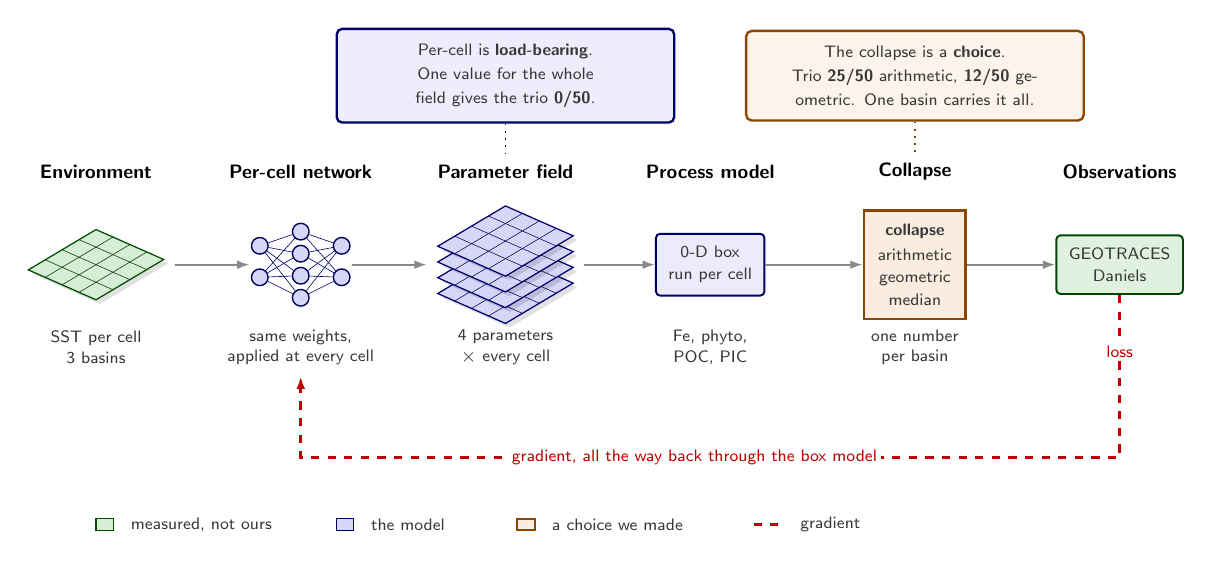
\begin{tikzpicture}[
  font=\sffamily,
  head/.style   ={font=\sffamily\bfseries\scriptsize, text=black, align=center},
  note/.style    ={font=\sffamily\fontsize{6}{7.4}\selectfont, text=myink, align=center},
  flow/.style   ={-{Latex[length=4.5,width=3.2]}, line width=0.8pt, draw=myink!60},
  neuron/.style ={circle, draw=myblue!45!black, fill=myblue!16, line width=0.5pt,
                  minimum size=6pt, inner sep=0},
  modelbox/.style={draw=myblue!50!black, line width=0.7pt, rounded corners=1.5pt,
                  fill=myblue!8, align=center, inner sep=4.5pt,
                  font=\sffamily\fontsize{6.5}{8}\selectfont, text=myink},
  choicebox/.style={draw=myorange!65!black, line width=1pt, fill=myorange!12,
                  align=center, inner sep=5pt,
                  font=\sffamily\fontsize{6.5}{8}\selectfont, text=myink},
  realbox/.style ={draw=mygreen!50!black, line width=0.7pt, rounded corners=1.5pt,
                  fill=mygreen!12, align=center, inner sep=4.5pt,
                  font=\sffamily\fontsize{6.5}{8}\selectfont, text=myink},
  callout/.style={rounded corners=2pt, align=center, inner sep=5.5pt, text width=3.9cm,
                  font=\sffamily\fontsize{6.5}{8.6}\selectfont, text=myink},
  tie/.style    ={line width=0.6pt, dotted},
]

% ============================================================ stage 1 : forcing (REAL)
\slabc{0}{0}{mygreen}
\node[head] at (0,1.18) {Environment};
\node[note]  at (0,-1.05) {SST per cell\\3 basins};

% ============================================================ stage 2 : network (MODEL)
\begin{scope}[shift={(2.6,0)}]
  \foreach \y [count=\i] in {0.24,-0.16} \node[neuron] (a\i) at (-0.52,\y) {};
  \foreach \y [count=\i] in {0.42,0.14,-0.14,-0.42} \node[neuron] (b\i) at (0,\y) {};
  \foreach \y [count=\i] in {0.24,-0.16} \node[neuron] (c\i) at (0.52,\y) {};
  \foreach \i in {1,2}\foreach \j in {1,...,4}
    \draw[draw=myblue!50!black, line width=0.22pt] (a\i) -- (b\j);
  \foreach \j in {1,...,4}\foreach \k in {1,2}
    \draw[draw=myblue!50!black, line width=0.22pt] (b\j) -- (c\k);
\end{scope}
\node[head] at (2.6,1.18) {Per-cell network};
\node[note]  at (2.6,-1.05) {same weights,\\applied at every cell};

% ============================================================ stage 3 : parameters (MODEL)
\foreach \dy in {-0.30,-0.10,0.10,0.30} { \slabc{5.2}{\dy}{myblue} }
\node[head] at (5.2,1.18) {Parameter field};
\node[note]  at (5.2,-1.05) {4 parameters\\$\times$ every cell};

% ============================================================ stage 4 : box (MODEL)
\node[modelbox] (box) at (7.8,0) {0-D box\\run per cell};
\node[head] at (7.8,1.18) {Process model};
\node[note]  at (7.8,-1.05) {Fe, phyto,\\POC, PIC};

% ============================================================ stage 5 : collapse (CHOICE)
\node[choicebox] (col) at (10.4,0)
  {\textbf{collapse}\\[1pt] arithmetic\\geometric\\median};
\node[head] at (10.4,1.18) {Collapse};
\node[note]  at (10.4,-1.05) {one number\\per basin};

% ============================================================ stage 6 : observations (REAL)
\node[realbox] (obs) at (13.0,0) {GEOTRACES\\Daniels};
\node[head] at (13.0,1.18) {Observations};
% "loss" is NOT a caption under this stage -- it is where the gradient originates, so it
% rides the red descent with a white fill that breaks the dashes. Sitting it at (13.0,-1.05)
% as a caption put it directly under the vertical run, and the line struck through it.

% ============================================================ flow, even pitch
\draw[flow] (1.00,0) -- (1.95,0);
\draw[flow] (3.25,0) -- (4.20,0);
\draw[flow] (6.20,0) -- (box.west);
\draw[flow] (box.east) -- (col.west);
\draw[flow] (col.east) -- (obs.west);

% ============================================================ gradient, the only red
% Routed orthogonally, not as a Bezier. Every other connector in this figure is a straight
% run; a lone curve reads as decoration rather than as the return path it is.
\draw[-{Latex[length=4.5,width=3.2]}, line width=0.9pt, draw=myred, dashed,
      line join=miter]
  (obs.south) -- (13.0,-2.45) -- (2.6,-2.45) -- (2.6,-1.42);
\node[note, text=myred, fill=white, inner sep=1.5pt] at (7.6,-2.45)
  {gradient, all the way back through the box model};
\node[note, text=myred, fill=white, inner sep=1.5pt] at (13.0,-1.10) {loss};

% ============================================================ the two results
% Both callouts sit directly above the stage they annotate and tie to it VERTICALLY.
% An earlier draft put this one at x=3.9 with a diagonal tie, which crossed the
% "Parameter field" heading and left it ambiguous whether it annotated the network or
% the field.
\node[callout, draw=myblue!50!black, line width=0.85pt, fill=myblue!7]
      (pA) at (5.2,2.40)
  {Per-cell is \textbf{load-bearing}.\\
   One value for the whole field gives the trio \textbf{0/50}.};
\draw[tie, draw=myblue!50!black] (pA.south) -- (5.2,1.42);

\node[callout, draw=myorange!65!black, line width=0.85pt, fill=myorange!8]
      (pB) at (10.4,2.40)
  {The collapse is a \textbf{choice}.\\
   Trio \textbf{25/50} arithmetic, \textbf{12/50} geometric. One basin carries it all.};
% Stops ABOVE the "Collapse" heading rather than running through it, matching the blue tie.
% Previously this ran pB.south -- col.north, straight over the label.
\draw[tie, draw=myorange!65!black] (pB.south) -- (10.4,1.42);

% ============================================================ legend
% Colour is doing semantic work here, so it needs declaring. Four roles, in the order they
% appear along the flow.
\begin{scope}[shift={(0,-3.30)}]
  \fill[mygreen!16, draw=mygreen!55!black, line width=0.45pt] (0,-0.075) rectangle ++(0.22,0.15);
  \node[note, anchor=west] at (0.32,0) {measured, not ours};

  \fill[myblue!16, draw=myblue!55!black, line width=0.45pt] (3.05,-0.075) rectangle ++(0.22,0.15);
  \node[note, anchor=west] at (3.37,0) {the model};

  \fill[myorange!12, draw=myorange!65!black, line width=0.7pt] (5.35,-0.075) rectangle ++(0.22,0.15);
  \node[note, anchor=west] at (5.67,0) {a choice we made};

  \draw[draw=myred, dashed, line width=0.9pt] (8.35,0) -- (8.72,0);
  \node[note, anchor=west] at (8.82,0) {gradient};
\end{scope}

\end{tikzpicture}
\end{document}
